% !TEX root = ../agglo_clust_review.tex

\section{Introduction}
%On possible selling story could be: currently many of the successful proposal-free instance segmentation methods rely on a final clustering step on a grid-graph with both short and long-range connections. So it is worth to study this problem in more details. 

\emph{Instance segmentation} is a task of computer vision consisting in assigning each pixel of an image to an object instance. %, where the number of instances is usually not known in advance. 
The most success in instance segmentation (IS) has been achieved by applying deep learning \cite{he2017mask,romera2016recurrent,liu2018affinity}. There are two main types of successful deep learning approaches to IS: proposal-based and proposal-free methods. Proposal-based methods consist of two steps: object detection, for example by finding bounding boxes, and assigning pixels to the detected objects \cite{he2017mask,dai2016instance,li2017fully}. Although these approaches have proven to be highly successful in instance segmentation competitions like MS COCO \cite{lin2014microsoft}, Pascal VOC2012 \cite{everingham2010pascal} and CityScapes \cite{cordts2016cityscapes}, they are not applicable to certain types of data, for example electron microscopy image volumes of neurons \cite{arganda2015crowdsourcing}, where objects are not approximated well by bounding boxes. 
% More motivation: They are at the same time limited by the quality of the object detection routine, which is hard to train on small datasets (but no ref for this)
Proposal-free methods perform IS by directly predicting pixel features and then using a clustering algorithm for grouping pixels into object instances \TODO{REFS}. In this work, we focus on a proposal-free method, where a Convolutional Neural Network (CNN) predicts affinities representing how likely it is for pairs of pixels to belong to the same instance. Recently, \cite{liu2018affinity} used this approach and achieved performances comparable to proposal-based methods on the Cityscapes dataset; \UPDATE{similarly, the method was used in \cite{wolf2018mutex} to achieve state-of-the-art results in a neuron segmentation challenge.} 

In this approach, the output of the CNN can be represented as a weighted grid graph such that each node represents a pixel of the image and the weights of the edges define interactions between the pixels. A graph clustering algorithm is then applied to cluster pixels into instances. The majority of clustering methods work with positive edge weights only, representing attractive interactions between the nodes. These methods require the user to specify the desired numbers of segments or a termination criterion (as in spectral clustering or iterated normalized cuts) or even a stronger version of supervision in terms of seeds (as in seeded watershed or random walker).  

A popular method for graph clustering is hierarchical clustering (HC) which creates an hierarchy of clusters. Agglomerative HC is a bottom-up approach starting with each node assigned to its own cluster and incrementally merging clusters while moving up the hierarchy \cite{lance1967general}. This method requires the user to choose a level in the cluster hierarchy defining the desired output clustering. 

Other clustering methods work with so-called \emph{signed graphs}, which include both positive and negative edge weights corresponding to attraction and repulsion between pixels \TODO{REFS}. The advantage of using signed graphs is that balancing attraction and repulsion allows us to perform the clustering without defining additional parameters. This can be done optimally by solving the so-called \emph{multicut optimization problem} or \emph{correlation clustering} \cite{kappes2011globally,chopra1991multiway}; however, this problem is NP-hard. For problems of considerable size, good approximations exist \cite{yarkony2012fast,pape2017solving}, and for even larger problems efficient greedy algorithms were recently proposed \cite{levinkov2017comparative,wolf2018mutex}.

Our main contribution is a framework for graph clustering that represents a generalization of agglomerative HC to graphs with both attractive and repulsive edge weights (see Figure \ref{fig:intro_figure} for a visual abstract). 
Various existing clustering algorithms, previously introduced in \cite{levinkov2017comparative,wolf2018mutex,lance1967general}, share the general procedure defined in our framework, but differ in the way in which the interaction between clusters is updated after each agglomeration step. In this work, we also introduce new variations of these algorithms by allowing the possibility of enforcing mutual-exclusion relationships between clusters during the agglomeration.  

Finally, \UPDATE{we test these different agglomerative clustering algorithms} on the task of instance segmentation both on the CREMI neuron segmentation challenge and the Cityscapes dataset, by comparing achieved scores, efficiency and robustness to noisy edge weights.

\TODO{Add chapters description} 




\begin{figure}[t]
\centering
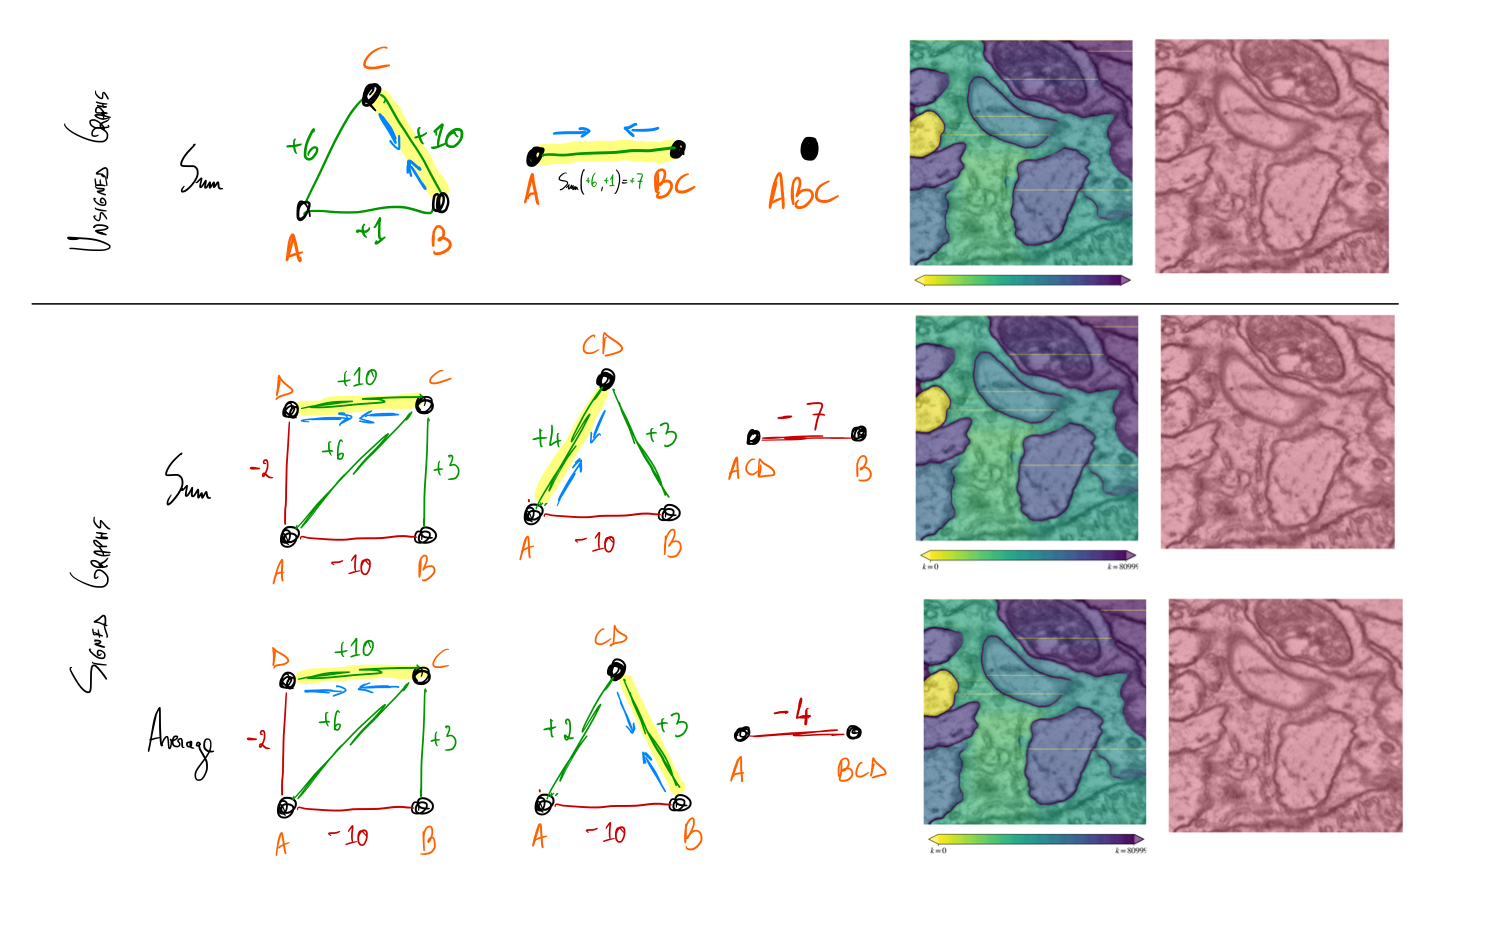
\includegraphics[width=\textwidth,trim=0.4in 1.2in 0.in 0.05in,clip]{./figs/intro_image.jpg} % left bottom right top
\caption{\small 
Intro image: explain algorithm, main ideas and contributions
\label{fig:intro_figure}}
\end{figure}
